\documentclass{beamer}
\useoutertheme{metropolis}
\useinnertheme{metropolis}
\usefonttheme{metropolis}
\usecolortheme{metropolis}
%
% Choose how your presentation looks.
%
% For more themes, color themes and font themes, see:
% http://deic.uab.es/~iblanes/beamer_gallery/index_by_theme.html
%
\mode<presentation>
{
  \usetheme{default}      % or try Darmstadt, Madrid, Warsaw, ...
  \usecolortheme{default} % or try albatross, beaver, crane, ...
  \usefonttheme{default}  % or try serif, structurebold, ...
  \setbeamertemplate{navigation symbols}{}
  \setbeamertemplate{caption}[numbered]
} 
\usepackage{movie15}
\usepackage{natbib}
\usepackage{hyperref}
\usepackage[english]{babel}
\usepackage[utf8x]{inputenc}
\usepackage{
	siunitx, % for SI notation
	wrapfig, % for figures with text next to them
	booktabs, % for better (alternative?) tables
  csquotes, % better biblatex
	cleveref, % better citations
	physics, % for better notation
	array, % for table stuff
}
\usepackage{stmaryrd}
% figures
\usepackage{graphicx}
\graphicspath{{fig/}} % can add more

% macros
\usepackage{xspace}
\newcommand*{\eg}{e.g.\@\xspace}
\newcommand*{\ie}{i.e.\@\xspace}
% cont'd
\makeatletter
\newcommand*{\etc}{%
    \@ifnextchar{.}%
        {etc}%
        {etc.\@\xspace}%
}
\makeatother

\title[Your Short Title]{Elements of neural network architecture}
\subtitle{Columbia Water Center - Neural Network Working Group}
\author{Luc Bonnafous \and James Doss-Gollin}
\institute{Columbia University}
\date{September $26^{th}$, 2017}
\begin{document}

\maketitle

% Uncomment these lines for an automatically generated outline.
\begin{frame}{Table of Contents}
  \setbeamertemplate{section in toc}[sections numbered]
  \tableofcontents[hideallsubsections]
\end{frame}

\section{Quick recap from last week}
\begin{frame}
	\frametitle{Chain Rule}
	Given a training sample $\vb{x}$ let’s compute the gradient of $f$ with respect to the weights $\vb{\theta}$.
	\begin{figure}
		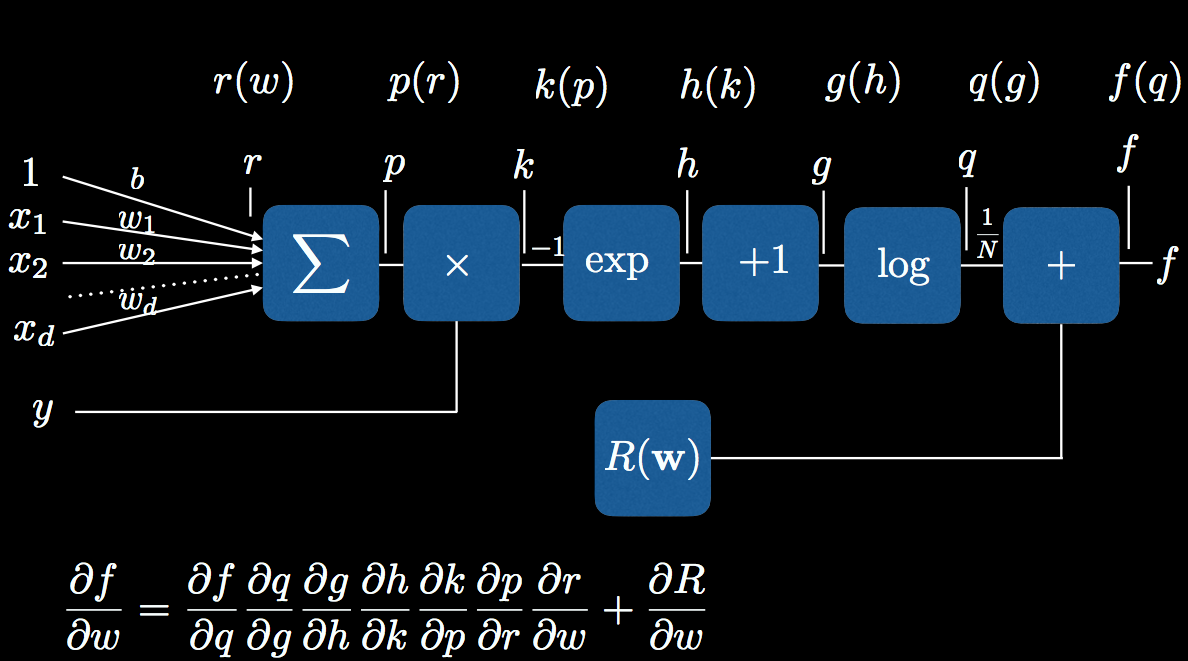
\includegraphics[width=\textwidth,height=0.5\textheight,keepaspectratio=true]{computational_derivatives.png}
		\caption{Chain rule for logistic regression example}
	\end{figure}
\end{frame}
\begin{frame}
	\frametitle{Gradient Descent}
	(There are more complicated ways to do this).
	Take our initial weights, choose a learning rate $\eta = 0.1$ say:
	\begin{equation}
		\vb{\theta}_{t+1} = \vb{\theta}_t - \eta \grad_{\vb{\theta}_t} f (\vb{\theta}_t)
	\end{equation}
\end{frame}

\begin{frame}
	\frametitle{Feedforward Network}
	We just need to generalize what we already learned.
	\begin{itemize}
		\item Let $y = f^*(\vb{x})$ be some function we don't know but want to approximate given data -- could be a classifier boundary!
		\item Try to learn parameters $\theta$ to approximate this
	\end{itemize}
	A feedforward network has \emph{no} feedback -- layers are composed of functions (``layers'') so that (\eg)
	\begin{equation}
		f (\vb{x}) = l^3(l^2(l^1(\vb{x})))
	\end{equation}
\end{frame}

\begin{frame}
	\frametitle{Over-fitting}
	\begin{figure}
		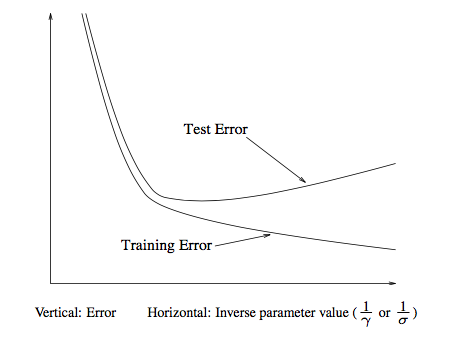
\includegraphics[width=\textwidth,height=0.85\textheight,keepaspectratio=true]{overfit_graph.png}
		\caption{Over-fitting can be a huge challenge!}
	\end{figure}
\end{frame}

\begin{frame}
	\frametitle{Ways to think of neural networks}
    \begin{itemize}
    	\item Sequence of layers mapping inputs into different "feature" spaces to learn meaningful feature combinations and draw conclusions
        \item Function approximators
        \item Ways to perform tasks such as classification, dimension reduction, and regression by learning from data
     \end{itemize}
\end{frame}

\section{A little more on backpropagation}
\begin{frame}
	\frametitle{Basic questions and framing}
    \begin{itemize}
    	\item How to learn multiple layers of features?
        \item We need to find a way to update each weight based on an error metric
        \item This method needs to be general enough to be applied to a variety of multi-layer networks with non-linear activation functions (we thus need an iterative method) 
        \item This method needs to be relatively efficient (better than difference-based methods based on weight perturbation)
        \item The idea is to use the error derivatives with respect to the activities of hidden units to evaluate the gradient the error function before applying some version of gradient descent
  \end{itemize}
\end{frame}

\begin{frame}
	\frametitle{General set-up}
  \begin{figure}       		        \includegraphics[width=\textwidth,height=1\textheight,keepaspectratio=true]{layer_l1.png}
 \caption{Adapted from Hagan et al., 2002}
 \end{figure}
\end{frame}

\begin{frame}
	\frametitle{Insisting on the different steps involved}
    \begin{itemize}
    	\item Training algorithms generally use a two step procedure to minimize the chosen error function, with adjustments made to the weights at each step
        \item The first steps evaluates the gradient of the error function relative to the weights: this is where backpropagation comes in (propagation of errors backwards through the network)
        \item Then adjustments to be made to the weights are computed using the derivatives obtained in the previous stage, often using a version of gradient descent 
  \end{itemize}
\end{frame}

\begin{frame}
	\frametitle{General set-up}
    \begin{itemize}
    	\item Let there be a network with $L$ layers in a given state, $N$ training examples. We write an input vector $X_n$, where $n \in \llbracket 1, N\rrbracket$, and the corresponding error $E_n$
        \item At the level of layer $l \in \llbracket 1, L\rrbracket $, we write $J$ the number of neurons, $K$ the number of inputs, $Z^{(l-1)}$ the vector of inputs, $Z^{(l)}$, the vector of outputs, $\vb{W^{(l)}} \in \mathbb{R}^{JxK}$, the weight matrix,  $w^{(l)}_{jk}$ the weight corresponding to input $k$ and neuron $j$, $a^{(l)}_j = \sum_{k}w^{(l)}_{jk}z^{(l-1)}_k$, and $h^{(l)}_j$ the activation function of neuron $j$ in layer $l$ (thus $h^{(l)}_j(a^{(l)}_j) = z^{(l)}_j$)
        \item We are looking for \color{red}
        \begin{equation}
        \pdv{E_n}{w^{(l)}_{jk}}
        \end{equation}
        \end{itemize}
\end{frame}

\begin{frame}
	\frametitle{Derivative computation}
    \begin{itemize}
    	\item For a given training example $X_n$, the error $E_n$ only depends on $w^{(l)}_{jk}$ through $a^{(l)}_j$, thus, using the chain rule:
        $\pdv{E_n}{w^{(l)}_{jk}} = \pdv{E_n}{a^{(l)}_j} \pdv{a^{(l)}_j}{w^{(l)}_{jk}}$
        
        \item We write \textcolor{red}{$\delta^{(l)}_j = \pdv{E_n}{a^{(l)}_j}$} the "error" for unit $j$
        \item We know that $\pdv{a^{(l)}_j}{w^{(l)}_{jk}}=z^{(l-1)}_k$, thus \textcolor{red}{$\pdv{E_n}{w^{(l)}_{jk}} = \delta^{(l)}_jz^{(l-1)}_k$}
        \item $z^{(l-1)}_k$ is known from forward propagation, and, if we write $M$ the number of neurons in the following layer, 
        \begin{equation}
          \delta^{(l)}_j = \sum_{m}\pdv{E_n}{a^{(l+1)}_m}\pdv{a^{(l+1)}_m}{a^{(l)}_j} = \color{red}h^{(l)'}_j\sum_{m}w^{(l+1)}_{mj}\delta^{(l+1)}_m
        \end{equation}where the $\delta_m$ are known from the previous steps of backpropagation (this is where the error is propagated backwards; for the top layer, $\delta_m=E_n$)
        \end{itemize}
\end{frame}


\begin{frame}
  \begin{figure}
  \includegraphics[width=\textwidth,height=0.9\textheight,keepaspectratio=true]{bp.png}
  \caption{Adapted from Bishop, 2006}
  \end{figure}
\end{frame}
\begin{frame}
	\frametitle{Derivative computation}
    \begin{itemize}
        \item In the case a batch is used at each time step, the gradient used will be $\pdv{E}{w^{(l)}_{jk}}=\sum_n\pdv{E_n}{w^{(l)}_{jk}}$
        \end{itemize}
\end{frame}

\begin{frame}
	\frametitle{Summary of what happens in practice}
    \begin{itemize}
    	\item A training example or a batch of training examples goes through the network, and the activations of all the units are recorded
        \item The errors of the output units are computed
        \item The $\delta$ are backpropagated using (4)
        \item The derivatives are computed
  \end{itemize}
\end{frame}

\begin{frame}
	\frametitle{A couple more points}
    \begin{itemize}
    	\item Backpropagation can be used to compute more stuff, such as the Hessian matrix that can be used for more efficient optimization procedures, pruning, re-training etc.
        \item What was presented above did not include regularization, early stopping, dropout which are used to prevent overfitting
        \item For Recurrent Neural Networks, the algorithm needs to be slightly modified (but not really)
        \item The question of no-derivable activation function has not been touched on either (ReLU layer) but is not a real issue in practice
  \end{itemize}
\end{frame}

\section{Activation functions}
\begin{frame}
	\frametitle{Canonical link functions}
	\begin{figure}
		\includegraphics[width=\textwidth,height=0.8\textheight,keepaspectratio=true]{transfer_functions.png}
		\caption{Source: Hagan et al., 2002}
	\end{figure}
\end{frame}

\begin{frame}
	\frametitle{Output layer}
    There is generally an obvious choice
	\begin{itemize}
    	\item Regression: identity
        \item Output strictly positive: softplus $y_k(a^{(K)}_k) = ln(1+ e^{(-a^{(K)}_k)})$
        \item Binary classification: logistic sigmoid
        \item Mutli-class classification: softmax: $y_k(a^{(K)}_k) = \frac{e^{(-a^{(K)}_k)}}{\sum_q(1+e^{(-a^{(K)}}_q)}$
    \end{itemize} 
    This choice often goes hand in hand with an error function:
    \begin{itemize}
    	\item Regression: sum of squared errors
        \item Binary classification: cross-entropy
        \item Mutli-class classification: cross-entropy
    \end{itemize} 
\end{frame}

\begin{frame}
	\frametitle{Hidden layers and link to backpropagation}
    \begin{itemize}
    	\item $tanh$ is preferred to the logistic sigmoid as it is zero-centered
        \item Recall $\delta^{(l)}_j = h^{(l)'}_j\sum_{m}w^{(l+1)}_{mj}\delta_m$\\
        For activation values outside a relatively small interval centered on zero, the gradient becomes very small, and thus almost no information on the error flows backward: the neuron  won't get updated despite the existence of errors in the  end, and the learning will become very slow or won't progress: {\color{red} vanishing gradient problem} (note: exploding gradient problem)
    \end{itemize}
\end{frame}

\begin{frame}
	\frametitle{ReLU}
	 \underline{Nowadays' standard:} ReLU (Rectified linear unit): $y_k(a^{(l)}_j) = max(0, a^{(l)}_j)$: it does not have the vanishing gradient problem, introduces non linearities, and its derivatives are easy to compute (more so that softplus, which is a smooth version of it)
     \begin{figure}
		\includegraphics[width=\textwidth,height=0.5\textheight,keepaspectratio=true]{ReLU.png}
		\caption{ReLU (blue) and softplus(green) - Source: Wikipedia}
	 \end{figure}
\end{frame}

\begin{frame}
	\frametitle{ReLU}
It still has some issues: it is not differentiable at zero, it is not zero-centered, and if the learning rate is high, it can reach states when it never gets to activate again (the neuron is dead).\break
Other version: Leaky ReLU  
\begin{figure}
		\includegraphics[width=\textwidth,height=0.5\textheight,keepaspectratio=true]{leakyrelu.png}
		\caption{Leaky ReLU - Source: Wangxin's Blog}
	 \end{figure}
\end{frame}

\section{Out of context cell and layer presentations}
\begin{frame}
	\frametitle{Basic Layer}
    \begin{itemize}
    \item This is your basic $\vb{z = h(WX+b)}$
    \end{itemize}
    \begin{columns}[T]
     \begin{column}{.5\textwidth}
    \begin{block}{}
    \begin{figure}
		\includegraphics[width=\textwidth,height=0.5\textheight,keepaspectratio=true]{basic_layer.png}
		\caption{Basic layer schematic - adapted from Hagan et al. 2002}
	 \end{figure}
    \end{block}
    \end{column}
    \begin{column}{.5\textwidth}
    \begin{block}{}
    \begin{itemize}
    	\item Keras
        keras.layers.core.Dense, keras.layers.core.Activation, keras.layers.core.Lambda
        \item Tensorflow
        tf.layers.dense, tf.matmul, tf.tanh, etc.
    \end{itemize}
    \end{block}
    \end{column}
    \end{columns}
\end{frame}

\begin{frame}
	\frametitle{Dropout layer}
    \begin{itemize}
    \item This type of cell drops some units of the incoming layer given a certain probability
    \end{itemize}
    \begin{columns}[T]
     \begin{column}{.5\textwidth}
    \begin{block}{}
    \begin{figure}
		\includegraphics[width=\textwidth,height=0.35\textheight,keepaspectratio=true]{dropout.jpg}
		\caption{Dropout layer schematic Source: Caffe framework}
	 \end{figure}
    \end{block}
    \end{column}
    \begin{column}{.5\textwidth}
    \begin{block}{}
    \begin{itemize}
    	\item Keras
        keras.layers.core.Dropout
        \item Tensorflow\\
        tf.layers.dropout
    \end{itemize}
    \end{block}
    \end{column}
    \end{columns}
    \begin{itemize}
    \item This is used to prevent overfitting
    \end{itemize}
\end{frame}

\begin{frame}
	\frametitle{Convolutional layer}
    \begin{itemize}
    \item Performs cross-correlations between filters and inputs
    \end{itemize}
    \begin{columns}[T]
     \begin{column}{.5\textwidth}
    \begin{block}{}
     \begin{figure}
		\includegraphics[width=\textwidth,height=0.5\textheight,keepaspectratio=true]{crosscorr.png}
		\caption{Cross-correlation between M1 and M2, - Source: Mathworks}
	 \end{figure}
    \end{block}
    \end{column}
    \begin{column}{.5\textwidth}
    \begin{block}{}
    \begin{itemize}
    	\item Keras
        keras.layers.convolutional .Conv2D
        \item Tensorflow\\
        tf.layers.conv2d
    \end{itemize}
    \end{block}
    \end{column}
    \end{columns}
\end{frame}

\begin{frame}
\frametitle{Convolutional layer}
  \begin{itemize}
      \item The goal is to detect features of given shapes by mapping the input sequence into a sequence of feature spaces to detect feature combinations
    \end{itemize}
    \begin{figure}
		\includegraphics[width=\textwidth,height=0.5\textheight,keepaspectratio=true]{conv_example1.png}
		\caption{Source: Adit Deshpande}
	 \end{figure}
\end{frame}

\begin{frame}
\frametitle{Convolutional layer}
  \begin{itemize}
      \item The goal is to detect features of given shapes by mapping the input sequence into a sequence of feature spaces to detect feature combinations
    \end{itemize}
    \begin{figure}
		\includegraphics[width=\textwidth,height=0.5\textheight,keepaspectratio=true]{conv_example2.png}
		\caption{Source: Adit Deshpande}
	 \end{figure}
\end{frame}

\begin{frame}
\frametitle{Convolutional layer}
  \begin{itemize}
      \item Stride controls the way the filter convolves around the input structure
   \end{itemize}
    \begin{figure}
		\includegraphics[width=\textwidth,height=0.5\textheight,keepaspectratio=true]{conv_stride.png}
		\caption{Source: Adit Deshpande}
	 \end{figure}
\end{frame}

\begin{frame}
\frametitle{Convolutional layer}
  \begin{itemize}
      \item Padding is here to adjust the output volume
    \end{itemize}
    \begin{figure}
		\includegraphics[width=\textwidth,height=0.5\textheight,keepaspectratio=true]{conv_padding.png}
		\caption{Source: Adit Deshpande}
	 \end{figure}
\end{frame}

\begin{frame}
	\frametitle{Pooling layers}
    \begin{itemize}
    \item Take a statistics from the output of a filter
    \end{itemize}
    \begin{columns}[T]
    \begin{column}{.5\textwidth}
    \begin{block}{}
    \begin{figure}
		\includegraphics[width=\textwidth,height=0.35\textheight,keepaspectratio=true]{max_pool.png}
		\caption{Max-pooling layer schematic - Source: Adit Deshpande}
	\end{figure}
    \end{block}
    \end{column}
    \begin{column}{.5\textwidth}
    \begin{block}{}
    \begin{itemize}
    	\item Keras
        keras.layers.pooling.MaxPooling2D, keras.layers.pooling.AveragePooling2D, etc.
        \item Tensorflow
       tf.layers.max\_pooling2d, etc.
    \end{itemize}
    \end{block}
    \end{column}
    \end{columns}
    \begin{itemize}
    \item Reduce the size of the info flowing if we don't really care about its exact location
    \end{itemize}
\end{frame}

\begin{frame}
	\frametitle{Locally-connected layer}
    \begin{itemize}
    \item Similar to convolution but with weights changing the filter weights for each position of the input
    \item Keras
        Keras.layers.local.LocallyConnected1D, Keras.layers.local.LocallyConnected2D
    \item Keep more spatial information
    \end{itemize}
\end{frame}

\begin{frame}
	\frametitle{"Deconvolution" layers}
    \begin{itemize}
    \item Go from something that has the shape of the output of some convolution to something that has the shape of its input while maintaining a connectivity pattern that is compatible with said convolution
    \end{itemize}    
\end{frame}

\begin{frame}
	\frametitle{"Deconvolution": unpooling}
    \begin{itemize}
    \item Uses both pooled maps and switches as inputs
    \end{itemize}
    \begin{figure}
		\includegraphics[width=\textwidth,height=0.8\textheight,keepaspectratio=true]{deconvolution.png}
		\caption{Unpooling - Source: Zeiler}
	\end{figure}
\end{frame}

\begin{frame}
	\frametitle{"Deconvolution": transpose convolution}
    \begin{itemize}
    \item Here the operation can be learned
    \end{itemize}
    \begin{columns}[t]
    \begin{column}{.6\textwidth}
    \begin{block}{}
    \begin{figure}
		\includegraphics[width=\textwidth,height=0.5\textheight,keepaspectratio=true]{tconv1.png}
		\caption{Transpose convolution - Source: Laboratoire d'Informatique des Systèmes d'Apprentissage}
	\end{figure}
    \end{block}
    \end{column}
    \begin{column}{.4\textwidth}
    \begin{block}{}
    \begin{itemize}
    	\item Keras
        conv2d\_transpose
        \item Tensorflow
       tf.layers.conv2d\_transpose
    \end{itemize}
    \end{block}
    \end{column}
    \end{columns}
\end{frame}

\begin{frame}
	\frametitle{"Deconvolution": transpose deconvolution}
    \begin{columns}[t]
    \begin{column}{.6\textwidth}
    \begin{block}{}
    \begin{figure}
		\includegraphics[width=\textwidth,height=0.5\textheight,keepaspectratio=true]{tconv2.png}
		\caption{Transpose convolution - Source: Laboratoire d'Informatique des Systèmes d'Apprentissage}
	\end{figure}
    \end{block}
    \end{column}
    \begin{column}{.4\textwidth}
    \begin{block}{}
    \begin{itemize}
    	\item Keras
        conv2d\_transpose
        \item Tensorflow
       tf.layers.conv2d\_transpose
    \end{itemize}
    \end{block}
    \end{column}
    \end{columns}
\end{frame}

\begin{frame}
	\frametitle{Basic recurrent layers}
    \begin{itemize}
    \item $\vb{z_t = h(WX_t+Ua_{t-1}+b)}$, $\vb{z_t = h(WX_t+Uy_{t-1}+b)}$
    \end{itemize}
    \begin{columns}[T]
    \begin{column}{.5\textwidth}
    \begin{block}{}
    \begin{figure}
		\includegraphics[width=\textwidth,height=0.35\textheight,keepaspectratio=true]{RNN1.png}
		\caption{Basic recurrent layer}
	\end{figure}
    \end{block}
    \end{column}
    \begin{column}{.5\textwidth}
    \begin{block}{}
    \begin{itemize}
    	\item Keras
        keras.layers.recurrent.
        SimpleRNN
        \item Tensorflow
       tf.contrib.rnn.BasicRNNCell
    \end{itemize}
    \end{block}
    \end{column}
    \end{columns}
    \begin{itemize}
    \item Keep information from previous steps, thus introducing memory in the system. Useful if inputs are not independent
    \end{itemize}
    
\end{frame}

\begin{frame}
	\frametitle{Basic recurrent layers}
    \begin{itemize}
  	\item Obviously, if you want to go too far back in time, it will screw up
    \item \href{https://deeplearning4j.org/lstm.html}{One representation}
    \item Another one:
    \end{itemize}
    \begin{figure}
		\includegraphics[width=\textwidth,height=0.35\textheight,keepaspectratio=true]{RNN2.png}
		\caption{Basic recurrent layer - Source: Christopher Colah}
	\end{figure}
\end{frame}

\begin{frame}
	\frametitle{Long short term memory layers}
    \begin{itemize}
    \item Choose how much of the previous info we keep
    \end{itemize}
    \begin{columns}[T]
    \begin{column}{.5\textwidth}
    \begin{block}{}
    \begin{figure}
		\includegraphics[width=\textwidth,height=0.5\textheight,keepaspectratio=true]{lstm.png}
		\caption{LSTM layer - Source: Christopher Colah}
	\end{figure}
    \end{block}
    \end{column}
    \begin{column}{.5\textwidth}
    \begin{block}{}
    \begin{itemize}
    	\item Keras
        keras.layers.recurrent.LSTM
        \item Tensorflow
       tf.contrib.rnn.BasicLSTMCell
    \end{itemize}
    \end{block}
    \end{column}
    \end{columns}
    \begin{itemize}
    \item Keep only useful information
    \end{itemize}
\end{frame}

\begin{frame}
	\frametitle{Long short term memory layers}
    \begin{figure}
		\includegraphics[width=\textwidth,height=0.5\textheight,keepaspectratio=true]{lstm2.png}
		\caption{LSTM layer - Source: Christopher Colah}
	\end{figure}
\end{frame}

\begin{frame}
	\frametitle{Long short term memory layers}
    \begin{columns}[T]
    \begin{column}{.5\textwidth}
    \begin{block}{}
    \begin{figure}
		\includegraphics[width=\textwidth,height=0.7\textheight,keepaspectratio=true]{lstm.png}
		\caption{LSTM layer - Source: Christopher Colah}
	\end{figure}
    \end{block}
    \end{column}
    \begin{column}{.5\textwidth}
    \begin{block}{}
    \begin{itemize}
    	\item $f_t = \sigma(W_fX_t+U_fh_{t-1}+b_f)$
        \item $i_t = \sigma(W_iX_t+U_ih_{t-1}+b_i)$
        \item $\tilde{C}_t = tanh(W_cX_t+U_ch_{t-1}+b_c)$
        \item $C_t = f_t*C_{t-1} + i_t*\tilde{C}_t$
        \item $o_t = \sigma(W_oX_t+U_oh_{t-1}+b_o)$
        \item $h_t = o_t*tanh(C_t)$
    \end{itemize}
    \end{block}
    \end{column}
    \end{columns}
\end{frame}

\begin{frame}
	\frametitle{Long short term memory layers}
    \begin{itemize}
    	\item Bi-directional RNN
        \item Peep-hole LSTM
        \item Convolutional LSTM
        \item Combining RNN and CNN, etc.
    \end{itemize}
\end{frame}

\section{Network examples}
\begin{frame}
	\frametitle{CNNs for image recognition}
    \begin{figure}
		\includegraphics[width=\textwidth,height=0.4\textheight,keepaspectratio=true]{cnn1.png}
		\caption{CNN structure - Source: Adit Deshpande}
	\end{figure}
    \begin{figure}
		\includegraphics[width=\textwidth,height=0.4\textheight,keepaspectratio=true]{cnn2.png}
		\caption{LeNEt structure - Source: LeCun 1998}
	\end{figure}
    \color{blue}\href{https://www.tensorflow.org/get_started/mnist/pros}{One more MNIST tutorial}
\end{frame}

\begin{frame}
	\frametitle{CNNs for image recognition}
    \begin{figure}
		\includegraphics[width=\textwidth,height=0.9\textheight,keepaspectratio=true]{conv_deconv_net.png}
		\caption{Conv/Deconv net structure - Source: Zeiler et al. 2013}
	\end{figure}
\end{frame}

\begin{frame}
	\frametitle{RNNs}
    \begin{figure}
		\includegraphics[width=\textwidth,height=0.9\textheight,keepaspectratio=true]{RNN3.png}
		\caption{RNN - Source: Reddit}
	\end{figure}
\end{frame}

\begin{frame}
	\frametitle{RNNs}
    \begin{figure}
		\includegraphics[width=\textwidth,height=1\textheight,keepaspectratio=true]{RNN4.png}
		\caption{RNN - Source: MLC}
	\end{figure}
\end{frame}

\begin{frame}
	\frametitle{More sophisticated image recognition}
    \begin{columns}[T]
    \begin{column}{.5\textwidth}
    \begin{block}{}
    \begin{figure}
		\includegraphics[width=\textwidth,height=0.5\textheight,keepaspectratio=true]{deep_mask.png}
		\caption{DeepMask - Source: Pinheiro et al. 2015}
	\end{figure}
    \end{block}
    \end{column}
    \begin{column}{.5\textwidth}
    \begin{block}{}
    \begin{figure}
		\includegraphics[width=\textwidth,height=0.5\textheight,keepaspectratio=true]{sharp_mask.png}
		\caption{SharpMask - Source: Pinheiro et al. 2016}
	\end{figure}
    \end{block}
    \end{column}
    \end{columns}
\end{frame}

\begin{frame}
	\frametitle{Autoencoder}
    \begin{figure}
		\includegraphics[width=\textwidth,height=1\textheight,keepaspectratio=true]{autoencoder.png}
		\caption{RNN - Source: UFLDL tutorial}
	\end{figure}
\end{frame}

\begin{frame}
	\frametitle{Last words}
    \begin{itemize}
    \item Not that many layer types in use, but variations of a couple
    \item Visualization
    \color{blue}\href{https://www.youtube.com/watch?v=AgkfIQ4IGaM}{DeepViz}
    \color{black}
    \item BNN
    \end{itemize}
\end{frame}

\begin{frame}
	\frametitle{References and resources}
    \underline{Books in the shared drive}
    \begin{itemize}
    \item Bishop 2006, Hagan 2002
    \end{itemize}
    \underline{Backpropagation}
	\begin{itemize}
    \item\href{http://jefkine.com/general/2016/09/05/backpropagation-in-convolutional-neural-networks/}{DeepGrid}
    \item \href{http://www.wildml.com/2015/10/recurrent-neural-networks-tutorial-part-3-backpropagation-through-time-and-vanishing-gradients/}{wildml}
    \item \href{http://neuralnetworksanddeeplearning.com/chap2.html}{neuralnetworksanddeeplearning}
    \item \href{http://colah.github.io/posts/2015-08-Backprop/}{Colah's blog}
    \end{itemize}
    \underline{CNNs \& RNNs}
    \begin{itemize}
    \item \href{https://adeshpande3.github.io/adeshpande3.github.io/A-Beginner's-Guide-To-Understanding-Convolutional-Neural-Networks/}{Deshpande's blog} 
    \item \href{http://warmspringwinds.github.io/}{Daniil's blog}
    \item \href{http://cs.nyu.edu/~fergus/drafts/utexas2.pdf}{NYU CS}
    \end{itemize}
\end{frame}





\end{document}


